\documentclass[../Thesis.tex]{subfiles}
\graphicspath{{\subfix{../figures/}}}
% \epstopdfsetup{outdir={../figures/}}
\usepackage{xr}
\externaldocument{C5 Results}
\begin{document}
% effects of scaling g_obs
% "bevis" for antagelse ikke holder for e.g. normalfordeling, men numerisk hvorfor det går godt??
% Hvad hvis man sætter entropi i diagonalen i stedet for 0? eller 1 hvis correlation. Undersøg numerisk.
% for at øge computer stabilitet kan G_obs skaleres til den har spektral radius mindre end 1. Spektrum/egenværdier numerisk mindre end 1
% $\rho\left(G_{obs}\right) < 1$ ??

% UNDERSØG: bruger original artikel at spektral radius af G_obs skal være mindre end 1? Det skal den ikke
% Det følger af proposition 5.3 / corrolary 5.2.1 at for en 1D manifold, under grænseværdien, at MI bare kan regnes som entropi for 1 af variablene (hvis det er 1-to-1??)

% Det er en vigtig del af correlation og MI at de virker for mixed variables. MI virker fordi continuert er grænsen for en diskretisering af en kontinuert variabel, så giver mening definitionsmæssigt at sammenligne kontinuert og diskret MI.

% \textcolor{red}{på et tidspunkt skal der laves et udvidet defintion af CE, så diskrete variable også kan tages med. Rent teknisk detalje, for bliver ikke brugt senere, kun til atomer som ikke behøver al den teori. inkluder også mix variable.}

% \textcolor{red}{Der skal argumenteres et sted for hvorfor vi bruger copula til at regne I ud. However, to make the calculations more robust and efficient we will use a closely related measure of dependence, namely CE which is defined as follows}

% The argument for calculating CE instead of MI are due to the finite volume integral and simpler integrand. In particular, using the copulas, we avoid the fraction $\frac{f(x_1,\dots,x_n)}{f_1(x_1)\dots f_n(x_n)}$ which could easily result in numerical instability e.g. when both $f$ and $f_i$s are close to 0.

% Correlation overholder faktisk antagelserne, men det gør MI ikke. Dog er correlation ikke altid et godt mål for forklaringsgrad, e.g. halvcirkel af perfekt forklaret punkter.

\chapter{Method}
\textcolor{red}{General introduction to metodeafsnittet og causalitet}

\section{Causal discovery}
In this section, we shall discuss the method for network deconvolution, originally proposed by \cite{Network-deconvolution-as-a-general-method-to-distinguish-direct-dependencies-in-networks}. The underlying problem is inferring direct effects and dependencies. From this, using prior information on the production setup, we shall be able to infer causal dependencies by directing the resulting edges from the network deconvolution (ND) algorithm. Particularly, the framework and general algorithm proposed by Feizi et al. stems from a graph-theoretic approach to the problem of inferring direct dependencies. \textcolor{blue}{Namely, suppose that observations are made of some properties such as levels and sojourn times of in this case a chemical process}. We shall represent these properties as vertices (nodes) $V$ and dependencies between properties as edges. Initially, when observing the vertices, we observe both direct and indirect effects. Particularly, a vertex $v_1$ might influence some other vertex $v_3$ through another vertex $v_2$ if $v_2$ depends on $v_1$ and $v_3$ of $v_2$. In this case, we will observe that $v_1$ influences $v_3$, but actually it is $v_2$ that has a direct influence on $v_3$. In graph-theoretical terms, we thus observe the transitive closure of the information that flows between vertices but want to infer the underlying network structure.

An important note on the algorithm to come is that we only use vertices that we have observed. Namely, the underlying structure might be as in \autoref{subfig:hidden nodes example unobserved} with an unobserved node/variable (named $U$ in this case). However, without any more assumptions or modelling choices we would (ideally) infer the network structure depicted in \autoref{subfig:hidden nodes example resulting graph}.
\begin{figure}[h]
    \centering
    \begin{subfigure}[t]{0.49\textwidth}
        \centering
        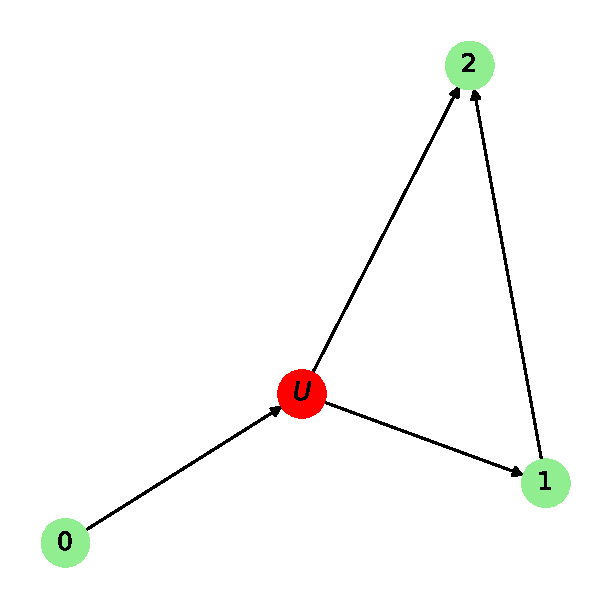
\includegraphics[width=\linewidth]{figures/ND examples/Hidden nodes/graph example w hidden.pdf}
        \caption{}
        \label{subfig:hidden nodes example unobserved}
    \end{subfigure}
    %
    \begin{subfigure}[t]{0.49\textwidth}
        \centering
        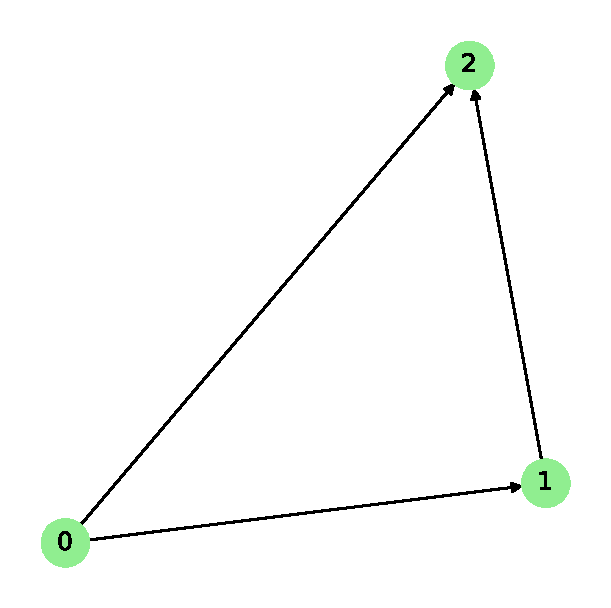
\includegraphics[width=\linewidth]{figures/ND examples/Hidden nodes/graph example wo hidden.pdf}
        \caption{}
        \label{subfig:hidden nodes example resulting graph}
    \end{subfigure}
    \caption{(a) An example of a causal structure depicted as a graph. When observing the network, only nodes $0$, $1$ and $2$ are observed/recorded. (b) The resulting inferred graph from observational data. Although this is not a complete picture of the true underlying dynamics of the system, if only the observed variables are of interest, this will be an equally proper representation of the system. Furthermore, in practice this means no further assumptions are made which can and can not be of desire. Namely, if prior information is accessible one might introduce new nodes in the inferred network.}
    \label{fig:hidden nodes example}
\end{figure}
With these initial comments, we proceed with the general setup and assumptions for network deconvolution based on observations.

\subsection{Setup and assumptions}\label{subsec:Setup and assumptions}
Suppose a set of $N$ random variables $(X_i)$ is given. The method presented in this section aims to discover direct relationships between pairs $X_i$ and $X_j$ for $i\neq j$. \textcolor{blue}{These relationships will be presented by a directed graph as in the previous section or an undirected graph in case the causal direction is either unknown or such an assumption on direction is not plausible}. In particular, we shall let each random variable $X_i$ be represented by a vertex in a graph. We will later discuss a way of directing edges such that a causal network may be discovered i.e. a directed acyclic graph that may be used for inference.

The method proposed by \cite{Network-deconvolution-as-a-general-method-to-distinguish-direct-dependencies-in-networks} then works as follows. Given an observed matrix $G_{obs} \in \mathbb{R}^{N \times N}$ of similarities between each pair of variables, we shall deduce a matrix $G_{dir} \in \mathbb{R}^{N \times N}$ of direct similarities between each pair of random variables $X_i$ and $X_j$. \textcolor{blue}{In particular, we wish to filter out indirect effects which we will denote by $G_{dir}$ defined as effects between pairs of variables that is the result of effects propagating through other variables}. The measure of similarity, can in practice be any desired measure such as correlation or mutual information which we will focus on in this thesis. See \autoref{seq:Information measures and computation} for a further discussion on these two measures and \autoref{sec:Copula based network discovery} for how to obtain such a matrix. Note that the algorithm presented will in theory work for non-symmetric measures as well such as \textit{Interaction information}, \textit{Directed information} and \textit{Normalized information}.

\textcolor{red}{illustration af hvordan algoritmen fungerer/formål}

The (direct) network is then presented by the discovered $G_{dir}$ containing only the direct effects i.e. interaction between pairs of variables which can be viewed as weights on the edges of the complete graph with nodes representing the random variables. As we shall see in \autoref{subseq:Robustness to noise}, the algorithm is somewhat robust to noise in the sense that we can ensure accuracy depending on the level of noise observed present in $G_{obs}$ and on the norm chosen (from a certain, although rather general, set of norms). \textcolor{blue}{Namely, if $G_{obs}$ is subject to noise, we find a bound on how different the inferred directed effects can be to the true direct effects using different matrix norms to measure this difference}. \textcolor{blue}{This hints to that a threshold on the inferred weights on the edges of the network might be a good idea to remove small inferred effects}. This is further supported by the facts that often only the most influential variables are of importance when trying to control the process.

The first assumption is that the observed matrix of co-dependence $G_{obs}$ may be expressed as
\begin{equation}
    G_{obs} = G_{dir} + G_{indir}
\end{equation}
Namely, that the direct and indirect effects can be added together to get the total and thus observed interdependence between each pair of variables. Often, this is not the case as we shall see later on. However, the error made from this assumption and the ones to be presented seem to be small enough that the discovered network accurately resemble the true underlying network.

The second and final assumption is that the indirect effects $G_{indir}$ can be computed in terms of $G_{dir}$. Namely, that
\begin{equation}
    G_{indir} = G_{dir}^2 + G_{dir}^3 + \dots
\end{equation}
i.e. that the observed \textit{information} exchanged on an edge $e_{ij}$ between nodes $X_i$ and $X_j$ is the sum of the second, third etc. order effects, each given by the information on the $n$-path (where $n$ is the order of the (diminishing) indirect effect) again assumed to be a sum of products. In other terms, the second order indirect effect between $X_i$ and $X_j$ (given as the $(i,j)$ element of $G_{dir}^2$) is the sum of products on edges $e_{ik}$ and $e_{kj}$ for all $k$
$$\left[G_{dir}^2\right]_{ij} = \sum_{k=1}^N e_{ik}\,e_{kj}$$
where $e_{ij}$ is the $(i,j)$ element of $G_{dir}$. \textcolor{blue}{This is of course not true in general, but through the error analysis in \autoref{subseq:Robustness to noise} and the examples in \autoref{chap:results} this is not necessarily a problem}. Immediately, we observe that $e_{ii}$ is of interest in terms of its physical meaning. The co-dependence between a random variable and itself might be somewhat ambiguous or even undefined depending on the measure. Thus, the notion of (non-existing) edges $e_{ii}$ will be of interest later on when using the method on controlled cases. We note that in $G_{obs}$ we shall in general set these elements to $0$.

Thus, from the above assumptions, it follows that we can express $G_{obs}$ as
\begin{equation}\label{eq:Network Informaiton Convolution}
    G_{obs} = G_{dir} + G_{dir}^2 + G_{dir}^3 + \dots = G_{dir} + G_{dir} \, G_{obs}
\end{equation}
Clearly, such a $G_{dir}$ must have spectral radius at most $1$ as otherwise, the above sum diverges and thus $G_{obs}$ will not exist. I.e. $\rho\left(G_{dir}\right) < 1$. Thus, assuming convergence we can rewrite the infinite series as
\begin{equation}\label{eq:Gobs from Gdir}
    G_{obs} = G_{dir} \left(I - G_{dir}\right)^{-1}
\end{equation}
It immediately follows that $G_{dir}$ is given by (can be proved by directly inserting the above expression for $G_{obs}$)
\begin{equation}\label{eq:Gdir from Gobs}
    G_{dir} = G_{obs} \left(I + G_{obs}\right)^{-1}
\end{equation}
Furthermore, if the measure of dependence between pairs of variables is symmetric, then so is $G_{obs}$ and hence diagonalizable by some orthogonal matrix $U$ and diagonal matrix $\Lambda_{obs}$ such that $G_{obs} = U \Lambda_{obs} U^T$ (with the columns of $U$ being right eigenvectors of $G_{obs}$). It follows that $G_{dir}$ can be expressed in a simple (and later computationally efficient) way
$$G_{dir} = U \Lambda_{dir} U^T$$
where $\Lambda_{dir} = \Lambda_{obs} \left(I + \Lambda_{obs}\right)^{-1}$ which is also a diagonal matrix.

We note that from the above one needs $\left( I + G_{obs}\right)^{-1}$ to be well-defined which is equivalent to $-1 \not\in \sigma_{G_{obs}}$ i.e. $-1$ is not an eigenvalue of $G_{obs}$. To see that this is indeed the case whenever $\rho\left(G_{dir}\right) < 1$, and that $I + G_{obs}$ is thus invertible we use \autoref{eq:Gobs from Gdir} and simplify
\begin{align*}
    I + G_{obs} & = I + G_{dir} \left(I-G_{dir}\right)^{-1}                                                \\
                & = \left(I-G_{dir}\right)\left(I-G_{dir}\right)^{-1} + G_{dir}\left(I-G_{dir}\right)^{-1} \\
                & = \left(I-G_{dir}\right)^{-1}
\end{align*}
which is clearly invertible. Furthermore, we note that under the assumption $\rho\left(G_{dir}\right) < 1$ we can not place any bound on the spectral radius of $G_{obs}$. Namely, if $v$ is a eigenvector of $G_{dir}$ with eigenvalue $\lambda$ such that $|\lambda|<1$, then $v$ is also an eigenvector of $G_{obs}$ as
$$G_{obs} v = \sum_{k=1}^\infty G_{dir}^k v = \sum_{k=1}^\infty \lambda^k v = \frac{\lambda}{1-\lambda} v$$
i.e. $\left(\frac{\lambda}{1-\lambda},v\right)$ is an eigenpair of $G_{obs}$ and since $\frac{\lambda}{1-\lambda} \in (-1/2, \infty)$ for $\lambda\in (-1,1)$ we can in general not bound the spectral radius of $G_{obs}$, although we should never observe an eigenvalue equal to or below $-1/2$ (which again proves that $-1$ is not an eigenvalue of $G_{obs}$).

As we shall later use some assumptions regarding causality i.e. directing the edges in the graph, we shall investigate the effect of letting $G_{obs}$ be a triangular matrix which corresponds to a directed acyclic graph. Namely, in the following, we show that given the existence of $G_{dir}$ (with necessary and sufficient conditions on $G_{obs}$ as given above), $G_{obs}$ is triangular if and only if $G_{dir}$ is triangular. Thus, by directing the observed similarity (by removing half the edge weights in $G_{obs}$), we also infer a directed graph $G_{dir}$.

Clearly, if $G_{dir}$ is triangular, so are the powers $G_{dir}^i$ for all $i\in\mathbb{N}$ and hence if the infinite sum $\sum_{i=1}^{\infty} G_{dir}^{i}$ converges, $G_{obs}$ is triangular as well. To show the other way, assume that $G_{obs}$ is triangular and is the result of a $G_{dir}$ with spectral radius smaller than $1$. By \autoref{eq:Gdir from Gobs}, $G_{dir}$ is triangular if the inverse of $I + G_{obs}$ is triangular (upper triangular if $G_{obs}$ is also upper triangular and similarly for lower triangular). This is indeed the case as in general, the inverse of a triangular matrix is also triangular provided that the diagonal elements are non-zero which is true as $ I + G_{obs}$ has only ones in the diagonal as we will later assume in \autoref{eq:Gobs matrix}. A simple proof of this is as follows. Without loss of generality, we assume that a matrix $T$ is upper triangular. Let $D$ be the diagonal elements of $T$ and $T_u$ be the remaining strictly upper triangular part of $T$ such that $T = D + T_{u}$. Then, assuming that $D$ has non-zero diagonal elements, $T = D \left(I + D^{-1}T_u\right)$ and hence, we have that
\begin{align*}
    T^{-1} & = \left(I + D^{-1}T_u\right)^{-1} D^{-1}               \\
           & = \sum_{i=0}^\infty \left(- D^{-1} T_u\right)^i D^{-1}
\end{align*}
which is clearly also upper triangular. Thus, we conclude that $G_{obs}$ is triangular if and only if $G_{dir}$ is (under the assumption $G_{dir}$ exists).

Finally, before discussing the implementation and analyzing the algorithm both analytically and through examples, we will take a closer look at the similarity measures that are to be used with this method and that in the end will make up the matrix $G_{obs}$. Namely, \textit{mutual information} and \textit{correlation}.


\section{Information measures and computation}\label{seq:Information measures and computation}
In this section we discuss two measures that can be used to construct the matrices of codependency from the previous section. Namely, we shall touch on correlation and discuss what one might choose to call Copula-based entropy. However, before discussing Copula entropy (CE) we first need to define what a copula is.

\subsection{Copula}
Given a set of $N$ random variables $X_1,\dots, X_d$, a copula is loosely speaking a distribution function with support $[0,1]^d$ incorporating the dependence structure between the random variables. Given a joint distribution function $F$ and (invertible) marginals $F_1,\dots,F_N$ we define a copula $C$ as
\begin{align*}
    F(x_1,\dots,x_N) & = \mathbb{P}\left(X_1\leq x_1,\dots, X_N\leq x_N\right)                                                                 \\
                     & = \mathbb{P}\left(F_1\left(X_1\right)\leq F_1\left(x_1\right),\dots, F_d\left(X_d\right)\leq F_d\left(x_d\right)\right) \\
                     & = C\left(F_1\left(x_1\right),\dots,F_N\left(x_N\right)\right)
\end{align*}
Letting $u_i = F_i\left(x_i\right) \in [0,1]$ it is clear that $C$ is a distribution function as described above \cite{Copula-handbook}. Furthermore, it follows that the marginals of $C$ are uniform as $F_i\left(X_i\right)$ is uniformly distributed. We thus define a copula in probabilistic terms as
\begin{definition}[Copula]\label{def:copula}
    A function $C:[0,1]^d \to [0,1]$ is called a copula if it has uniform marginals and is a distribution function for a $d$-dimensional random vector $\mathbf{X}$.
\end{definition}
An important and fundamental theorem of copulas for especially continuous random variables where the marginals are also continuous functions is stated by Sklar:
\begin{theorem}[Sklar's theorem] \label{thm: Sklar}
    For a random vector $\boldsymbol X$ with CDF $F$ and univariate marginal CDFs $F_1, \dots, F_d$. There exists a copula $C$ such that
    \begin{equation}\label{eq:sklar}
        F(x_1,\dots,x_d) = C(F_1(x_1), \dots, F_d(x_d))
    \end{equation}
    If $X$ is continuous, $C$ is unique; otherwise $C$ is uniquely determined on the Cartesian product of the ranges of distribution functions $F_i$, $\prod \text{Ran}\left(F_i\right)$.
\end{theorem}
Note that the last statement for non-continuous random variables can be made unique by instead using subcopulas, a generalization of copulas with domain $I$ only a subdomain of the unit hypercube $\mathbb{I}^d = [0,1]^d$ containing all faces of the unit hyper cube. However, there are infinitely many ways of extending such a subcopula to a copula $C$\cite{Copula-modeling-for-discrete-random-vectors}. In our case, this means that for discrete and/or mixed variables, we will later have to work around this non-uniqueness when calculating mutual information. The example made by Geenens\cite{Copula-modeling-for-discrete-random-vectors} is a bivariate random vector of independent variables $X \sim \text{Bern}\left(\pi_X\right)$ and $Y\sim \text{Bern}\left(\pi_Y\right)$. The support of $F_X$ and $F_Y$ is then $\{0, 1-\pi_X\}$ and $\{0, 1-\pi_Y\}$ respectively. Due to the restriction on the boundary of the unit square, the only unique point of a copula $C$ is then $(1-\pi_X, 1-\pi_Y)$, and by independence we must have
$$C\left(1-\pi_X, 1-\pi_Y\right) = (1-\pi_X)( 1-\pi_Y)$$
Geenens then proceed to define an uncountable set of copulas that fulfill the above criterion which further illustrates that the basic concepts of copulas are not well suited for discrete random vectors. Note that in the article it is however argued how one can extend the concept to a more general concept that works for mixed variables.

From \autoref{eq:sklar} we see that a copula is thus simply just a function that \textit{couples} the marginals of a random vector to the joint distribution. The following corollary follows immediately
\begin{corollary}[Coordinate transformation] \label{coro: Coordinate transformation}
    Under the assumptions of \autoref{thm: Sklar}, given any set $(T_1, \dots, T_d)$ of strictly increasing functions, if $C$ is a copula of $(X_1,\dots, X_d)$ then it is also a copula of $(T_1(X_1), \dots, T_d(X_d))$.
\end{corollary}
\begin{proof}
    Suppose $(X_1 , \dots , X_d)$ permits a copula $C$ and let $T_i$ be given as stated. Consider coordinate wise the result of the transformation $Y_i = T_i(X_i)$ and consider the CDF $F_{Y_i}(y_i)$
    \begin{align*}
        F_{Y_i}(y_i) & = \mathbb{P}\left(Y_i \leq y_i\right)                      \\
                     & = \mathbb{P}\left(T_i^{-1}(Y_i) \leq T_i^{-1}(y_i)\right)  \\
                     & = \mathbb{P}\left(X_i \leq T_i^{-1}\left(y_i\right)\right) \\
                     & = F_{X_i}\left(T_i^{-1}\left(y_i\right)\right)
    \end{align*}
    The above is easily generalized for a joint distribution as well. Thus, by the existence of a Copula $C$ for $\boldsymbol{X}$
    \begin{align*}
        F_{\boldsymbol Y}(y_1, \dots, y_d) & = F_{\boldsymbol X} \left(T_1^{-1}\left(y_1\right),\dots , T_d^{-1}\left(y_d\right)\right)   \\
                                           & = C\left( F_{X_1}(T_1^{-1}\left(y_1\right)), \dots, F_{X_d}(T_d^{-1}\left(y_d\right))\right) \\
                                           & = C\left( F_{Y_1}(y_1), \dots, F_{Y_d}(y_d)\right)
    \end{align*}
    where Sklar's theorem have been used for the second equality. The above shows that $C$ is indeed also a Copula for $\boldsymbol Y = \left(T_1(X_1), \dots, T_d(X_d)\right)$.
\end{proof}
The above corollary is actually equivalent with a seemingly stronger statement and follows easily
\begin{proposition}
    Since $T_i$ is strictly increasing, the inverse $T_i^{-1}$ exists and is also strictly increasing. Thus, the above implication is bidirectional and hence for strictly increasing functions $T_i$, $C$ is a copula of $\left(X_1,\dots,X_d\right)$ if and only if it is a copula of $\left(T_1(X_1),\dots, T_d(X_d)\right)$.
\end{proposition}












\subsection{Mutual information and Copula entropy}
In this section we introduce Copula entropy as done in \cite{Nonparametric-copula-entropy-and-network-deconvolution-method-for-causal-discovery-in-complex-manufacturing-systems} and see how it actually is equal to the well known mutual information (multiplied by $-1$) and hence as a corollary that mutual information is independent of marginals. The name comes from the general definition of (differential) entropy as we shall see shortly. However, first we define mutual information between a set of random variables
\textcolor{blue}{
    \begin{definition}[Mutual information]\label{def:mutual information}
        For a random vector $\boldsymbol{X} = \{X_i\}$, we define the mutual information as
        $$I(\boldsymbol{X}) = \mathbb{E}\left[\log_b \left(\frac{f(\boldsymbol X)}{\prod_i f_i (X_i)}\right)\right]$$
        % $$I(\boldsymbol{X}) = \sum_{\boldsymbol{x} \in \mathcal{X}} f(\boldsymbol{x}) \, \log_b\left(\frac{f(\boldsymbol{x})}{\prod_{i} f_i\left(x_i\right)}\right)$$
        where $f$ is the joint density function with marginals $f_i$ of the random vector $\boldsymbol{X}$.
        % If $\boldsymbol X$ is discrete and $f$ is the joint probability mass function with marginals $f_i$. Similarly, for continuous random vectors with $f$ the joint probability density function we define
        % $$I(\boldsymbol{X}) = \int_{\mathcal{X}} f(\boldsymbol{x}) \, \log_b\left(\frac{f(\boldsymbol{x})}{\prod_{i} f_i\left(x_i\right)}\right)\, d\boldsymbol{x}$$
        The base of the logarithm $b$ is often chosen to be $2$, $e$ or $10$ although the choice is unimportant as all logarithms are equivalent up to a scaling factor.
    \end{definition}
}
We note that later on, as the choice of $b$ will result in a scaling of $G_{obs}$, but we will also introduce a scaling parameter $\alpha$ for $G_{obs}$ to both ensure the convergence of the algorithm and to control higher order effects, we shall in general choose $b = e$.

An important property of mutual information is that the continuous version is the limit of the discrete mutual information for random (continuous) vector discretized as the mesh size goes to zero i.e. recovering the continuity of the random vector. This is discussed in \autoref{subsec:limit entropy and MI}. For now, we proceed with the definition of (joint) entropy for both discrete and continuous random vectors.
\textcolor{blue}{
    \begin{definition}[Entropy]\label{def:entropy}
        The (joint) entropy of a random vector $\boldsymbol{X}$ is defined as
        % $$H\left(\boldsymbol{X}\right) = - \sum_{\boldsymbol{x}\in \mathcal{X}} f(\boldsymbol{x}) \, \log_b f(\boldsymbol{x})$$
        $$H\left(\boldsymbol{X}\right) = - \mathbb{E}\left[\log_b f(\boldsymbol X)\right]$$
        In case of a discrete random vector, this is called the Shannon entropy while for continuous random vectors, this is called differential entropy and is often denoted as $h\left(\boldsymbol X\right)$ instead of $H\left(\boldsymbol X\right)$.
    \end{definition}
}
% And likewise for continuous random vectors, which we name differential entropy
% \begin{definition}[Differential entropy]\label{def:differential entropy}
%     The (joint) differential entropy defined for a continuous random vector $\boldsymbol{X}$ is defined as
%     $$h(\boldsymbol{X}) = - \int_{\mathcal{X}} f\left(\boldsymbol{x}\right) \, \log_b f\left(\boldsymbol{x}\right) \, d\boldsymbol{x}$$
% \end{definition}
We note the need for two separate notations of entropy as differential entropy is not the limit of Shannon entropy in the way mutual information is. Again, this is further discussed in \autoref{subsec:limit entropy and MI}.
% However, they are both equal to the expectation $\mathbb{E}\left(\log f\left(\boldsymbol X\right)\right)$.

Before discussing Copula entropy (CE), we note a very useful relation between entropy and mutual information. Indeed, we shall later use this to show that mutual information in the continuous version is the limit of the discretization.
\begin{lemma}[Mutual information and entropy relation]\label{lemma:mutual information and entropy relation}
    For a continuous random vector $\boldsymbol{X}$, the (joint) mutual information $I\left(\boldsymbol{X}\right)$ can be decomposed into a sum of differential entropies as
    $$I\left(\boldsymbol{X}\right) = \sum_{i=1}^{d} h(X_i) - h\left(\boldsymbol{X}\right)$$
    where $d$ is the dimension of $\boldsymbol{X}$. The same is true for discrete variables but with entropy $H$ instead of differential entropy $h$.
\end{lemma}
\textcolor{blue}{\begin{proof}
        This follows immediately from the definition of mutual information and entropy:
        $$\mathbb{E}\left[\log_b \frac{f\left(\boldsymbol X\right)}{\prod_i f_i\left(X_i\right)}\right] = \mathbb{E}\left[\log_b f\left(\boldsymbol X\right) \right] - \sum_i \mathbb{E}\left[\log_b f_i \left(X_i\right)\right]$$
        % The proof is identical for discrete and continuous random vectors. Hence, we only show the proof in the continuous case. By direct computation
        % \begin{align*}
        %     I\left(\boldsymbol{X}\right) & = \int_{\mathcal{X}} f\left(\boldsymbol{x}\right) \, \log_b f\left(\boldsymbol{x}\right) \, d\boldsymbol{x} - \sum_{i = 1}^{d} \int_{\mathcal{X}} f\left(\boldsymbol{x}\right) \, \log_b f_i\left(x_i\right) \, d\boldsymbol{x} \\
        %                                  & = \int_{\mathcal{X}} f\left(\boldsymbol{x}\right) \, \log_b f\left(\boldsymbol{x}\right) \, d\boldsymbol{x} - \sum_{i = 1}^{d} \int_{\mathcal{X}_i} f_i\left(\boldsymbol{x}\right) \, \log_b f_i\left(x_i\right) \, d x_i       \\
        %                                  & = \sum_{i=1}^{d} h\left(X_i\right) - h\left(\boldsymbol{X}\right)
        % \end{align*}
    \end{proof}}
With the definitions of mutual information and entropy we are finally ready to introduce Copula entropy.
\begin{definition}[Copula entropy]\label{def:copula entropy}
    For a continuous random vector $\boldsymbol{X}$ with a uniquely defined Copula $C$, and Copula density $c$, we define the Copula entropy $CE$ of $\boldsymbol{X}$ as
    $$CE\left(\boldsymbol{X}\right) = h\left(\boldsymbol U\right)$$
    where $\boldsymbol U$ has density $c$. In particular,
    $$CE\left(\boldsymbol{X}\right) = - \mathbb{E}\left[\log_b c\right]$$
    % $$CE\left(\boldsymbol{X}\right) = - \int_{[0,1]^d} c\left(\mathbf{u}\right) \, \log_b c\left(\mathbf{u}\right) \, d\mathbf{u}$$
\end{definition}
As stated above, Copula entropy is actually equal to the negative mutual information which we state as a theorem
\begin{theorem}[Equality of Copula entropy]\label{thm:copula entropy equals mutual information}
    For a continuous random vector $\boldsymbol{X}$, the Copula entropy $CE$ is equal to the negative joint mutual information of $\boldsymbol{X}$
    $$CE\left(\boldsymbol{X}\right) = - I\left(\boldsymbol{X}\right)$$
\end{theorem}
\begin{proof}
    By \autoref{thm: Sklar}, letting $x_i = F_i^{-1}\left(u_i\right)$, we can relate the copula density to the joint density of $\boldsymbol{X}$ and its marginals
    \begin{align*}
        c(u_1,\dots , u_n) & = \frac{\partial}{\partial \mathbf{u}} C(u_1,\dots,u_n)                                                                                                                   \\
                           & = \frac{\partial}{\partial \mathbf{u}} F\left(F_1^{-1}\left(u_1\right), \dots, F_n^{-1}\left(u_n\right)\right)                                                            \\
                           & = f\left(F_1^{-1}\left(u_1\right),\dots, F_1^{-1}\left(u_n\right)\right) \frac{1}{f_1\left(F_1^{-1}\left(u_1\right)\right)\dots f_n\left(F_1^{-1}\left(u_d\right)\right)}
    \end{align*}
    It follows directly that
    \begin{align*}
        -CE\left(\boldsymbol{X}\right) & = \int_{[0,1]^d} c\left(\boldsymbol{u}\right) \log c\left(\boldsymbol{u}\right) \, d\boldsymbol{u}                                                                                                                        \\
                                       & =  \int_{\mathcal{X}} \frac{f(\boldsymbol{x})}{\prod_{i=1}^{d} f_i\left(x_i\right)} \log\left(\frac{f(\boldsymbol{x})}{\prod_{i=1}^{d} f_i\left(x_i\right)}\right) \prod_{i=1}^{d} f_i\left(x_i\right) \, d\boldsymbol{x} \\
                                       & = \int_{\mathcal{X}} f(\boldsymbol{x}) \log\left(\frac{f(\boldsymbol{x})}{\prod_{i=1}^{d} f_i\left(x_i\right)}\right) \, d\boldsymbol{x}                                                                                  \\
                                       & = I\left(\boldsymbol{X}\right)
    \end{align*}
    \textcolor{blue}{where the third equality follows from a change of variables with the trivial substitution $u_i = F_i(x_i)$ such that $du_i = f_i(x_i)\,dx_i$. This concludes the proof.}
\end{proof}
Finally, before moving on to correlation as a measure of similarity, we discuss what happens in the limit of mutual information and entropy as we shall later need this as arguments for numerical stability.


\subsection{Entropy and mutual information in the limit}\label{subsec:limit entropy and MI}
In this section, we shall discuss the differences between entropy and differential entropy and observe how this difference cancels when computing mutual information. In fact, we shall see that mutual information defined for continuous random vectors is the limit of the discrete version which will be useful later when implementing the algorithm.

First, although one may think differential entropy this as the limit of (discrete) entropy, this is not the case. Namely, consider the support of $f(x)$ (here assumed to be the entire real line) binned into intervals i.e. a discretization of the continuous random variable $X$, which we shall denote $X^{\Delta}$. To make notation simpler, we shall bin into equal-sized intervals of width $\Delta$. Then, for each interval $[i\Delta, (i+1)\Delta]$ for $i \in \mathbb{Z}$, there exists an $x_i$ such that the probability mass on this interval is represented by this $x_i$:
\textcolor{blue}{
    \begin{equation}\label{eq:one dim discretization}
        \mathbb{P}\left(X^{\Delta} = x_i\right) = f(x_i) \Delta = \int_{i\Delta}^{(i+1)\Delta} f(x) \, dx
    \end{equation}
}
Clearly, this discretization is a valid distribution as
$$\sum_{i\in\mathbb{Z}} f(x_i) \Delta = \int_{\mathbb{R}} f(x) \, dx = 1$$
and in the limit, as $\Delta \to 0$ we recover the original distribution $f(x)$. However, if we try to calculate the entropy of this discretization, denoted by $H^{\Delta}$, we get a diverging limit
\begin{align*}
    H^{\Delta} & = \sum_{i\in\mathbb{Z}} f(x_i) \Delta \log{f(x_i) \Delta}                                             \\
               & = \sum_{i\in\mathbb{Z}} f(x_i) \Delta \log{f(x_i)} + \sum_{i\in\mathbb{Z}} f(x_i) \Delta \log{\Delta} \\
               & = \sum_{i\in\mathbb{Z}} f(x_i) \Delta \log{f(x_i)} + \log{\Delta}
\end{align*}
Clearly, the first term in the above expression converges to the differential entropy $h\left(X\right)$ as $\Delta \to 0$ whereas $\log{\Delta} \to - \infty$ i.e. the expression diverges altogether when differential entropy is well-defined.

A similar argument for the joint entropy between the discretization of $X_1$ and $X_2$ (and in principle to any number of dimensions), denoted by $H^{\Delta}_{12}$, results in
$$H^{\Delta}_{12} = \sum_{i,j \in \mathbb{Z}} f\left(x_1^{(i)}, x_2^{(j)}\right) \Delta_1 \Delta_2 \log{f\left(x_1^{(i)}, x_2^{(j)}\right)} + \log{\Delta_1} + \log{\Delta_2}$$
where $x_1^{(i)}\in[i\Delta_1, (i+1)\Delta_1)$ and $x_2^{(j)}\in [j\Delta_2, (j+1)\Delta_2)$ are defined such that
$$f\left(x_1^{(i)}, x_2^{(j)}\right)\Delta_1 \Delta_2 = \int_{j\Delta_2}^{(j+1)\Delta_2}\int_{i\Delta_1}^{(i+1)\Delta_1} f(x_1,x_2) \, dx_1 dx_2,\quad \forall i,j\in\mathbb{Z}$$
Note that clearly $\left(x_1^{(i)},x_2^{(j)}\right)$ exists for all $i,j\in \mathbb{Z}$. Again, the joint entropy diverges however, when computing the mutual information, we see that the diverging terms cancel. Namely, from \autoref{lemma:mutual information and entropy relation}
\begin{align*}
    I^{\Delta}_{12} & = H^{\Delta}_1 + H^{\Delta}_2 - H^{\Delta}_{12}                                                                                                                                                                     \\
                    & = \sum_{i\in\mathbb{Z}} f_1\left(\tilde{x}_1^{(i)}\right) \Delta_1 \log{f_1\left(\tilde{x}_1^{(i)}\right)} + \log{\Delta_1}                                                                                         \\
                    & \quad + \sum_{j\in\mathbb{Z}} f_2\left(\tilde{x}_2^{(j)}\right) \Delta_2 \log{f_2\left(\tilde{x}_2^{(j)}\right)} + \log{\Delta_2}                                                                                   \\
                    & \quad - \sum_{i,j\in\mathbb{Z}} f\left(x_1^{(i)},x_2^{(j)}\right) \Delta_1 \Delta_2 \log{f\left(x_1^{(i)},x_2^{(j)}\right)} - \log{\Delta_1 \Delta_2}                                                               \\
                    & =\sum_{i\in\mathbb{Z}} f_1\left(\tilde{x}_1^{(i)}\right) \log{f_1\left(\tilde{x}_1^{(i)}\right)}\Delta_1 + \sum_{j\in\mathbb{Z}} f_2\left(\tilde{x}_2^{(j)}\right)  \log{f_2\left(\tilde{x}_2^{(j)}\right)}\Delta_2 \\
                    & \quad -\sum_{i,j\in\mathbb{Z}} f\left(x_1^{(i)},x_2^{(j)}\right) \log{f\left(x_1^{(i)},x_2^{(j)}\right)} \Delta_1 \Delta_2                                                                                          \\
                    & \to h(X_1) + h(X_2) - h(X_1,X_2)\; \text{as}\; \Delta_1,\Delta_2 \to 0
\end{align*}
Thus, the limit of the mutual information for discrete random variables is indeed the mutual information defined for continuous random variables and can be computed either as the limit of discretizing the probability density function and then computing entropies or just using the initial definition for (discrete) mutual information in \autoref{def:mutual information}.

Before continuing, we discuss the case where $X_1$ is equal to $X_2$. In this case, discretizing with a common $\Delta$ we have that
$$f\left(x_1^{(i)}, x_2^{(j)}\right)\Delta^2 = \int_{j\Delta}^{(j+1)\Delta}\int_{i\Delta}^{(i+1)\Delta} f(x_1,x_2) \, dx_1 dx_2,\quad \forall i,j\in\mathbb{Z}$$
Clearly, the above integral is $0$ for $i\neq j$. Although $f(x_1,x_2)$ is not well-defined in the usual functional sense, extending to distribution, we might write $f(x_1,x_2) = f(x_2 | x_1) f(x_1)$. In terms of distributions, it works to put $f(x_2 | x_1) = \delta(x_2 - x_1)$ where $\delta$ is the \textit{Dirac delta} distribution, as then $\int_{\mathbb{R}} f(x_1,x_2) \, dx_2 = f(x_1)$ and $f(x_1, x_2)$ is "$0$" when $x_1 \neq x_2$. I.e. the right marginals and probability mass $1$. Then, when calculating the above integral, we get that
\begin{align*}
    f\left(x_1^{(i)}, x_1^{(i)}\right)\Delta^2 & = \int_{i\Delta}^{(i+1)\Delta}\int_{i\Delta}^{(i+1)\Delta} f(x_1,x_2) \, dx_1 dx_2 \\
                                               & = \int_{i\Delta}^{(i+1)\Delta} f\left(x_1\right)\, dx_1                            \\
                                               & = f\left(\tilde{x}_1^{(i)}\right)\Delta
\end{align*}
Thus, when calculating $I^{\Delta}_{1,2}$ we obtain
\begin{align*}
    I^{\Delta}_{1,2} & = \sum_{i\in\mathbb{Z}} f_1\left(\tilde{x}_1^{(i)}\right) \log{f_1\left(\tilde{x}_1^{(i)}\right)}\Delta + \sum_{j\in\mathbb{Z}} f_2\left(\tilde{x}_2^{(j)}\right)  \log{f_2\left(\tilde{x}_2^{(j)}\right)}\Delta \\
                     & \quad - \sum_{i\in\mathbb{Z}} f_1\left(\tilde{x}_1^{(i)}\right) \log{f_1\left(\tilde{x}_1^{(i)}\right)}\Delta - \log \Delta                                                                                      \\
                     & \to \infty \;\text{as}\; \Delta \to 0
\end{align*}
Thus in practice, it would not make much sense to compare equal variables or even a random vector only defined on a lower dimensional manifold as we would get an infinite Copula entropy.





\subsection{Correlation}
At this point, we have a good understanding of Copula entropy/mutual information for calculations later on. However, another typical measure of similarity is correlation which is easily estimated from sample data. However, in this section we show that in general, we can not compute the correlation coefficient from a Copula which we saw above is the case for mutual information. Namely, given a copula $C$ for some set of random variables $\{X_i\}_{i\in I}$ indexed by finite $I$, one can not calculate $\rho$ between any pair $(X_i ,X_j)$, $i\neq j$ from the copula. This is easily shown by the following argument.

First, note that from \autoref{coro: Coordinate transformation}, $C$ is also a copula for $Z_i \coloneq \left( X_i - \mu_i\right) / \sigma_i$ for $i \in I$ where $\mu_i = \mathbb{E}[X_i]$ and $\sigma_i = \sqrt{\text{Var} \, X_i}$. Clearly, the correlation coefficient for $Z_i$ and $Z_j$ is the same as between $X_i$ and $X_j$. We thus proceed trying to calculate the correlation between any pair $Z_i$ and $Z_j$.
\begin{align*}
    \rho_{ij} & = \int\int_{\mathbb{R}^2} z_i z_j f_{ij}(z_i,z_j) \, dz_i \, dz_j                       \\
              & = \int\int_{[0,1]^2} F_i^{-1}(u_i) \, F_j^{-1}(u_j) \, c_{ij}(u_i, u_j) \, du_i \, du_j
\end{align*}
where $c_{ij}$ density version of the copula defined for $X_i$ and $X_j$ and $F_i$ and $F_j$ are the marginals of $Z_i$ and $Z_j$ with mean $0$ and variance $1$. From the above, it is then clear for a fixed, non-constant copula $C$, the correlation depends on the marginals of $X_i$ and $X_j$. Also, we see that a constant copula density (only admissible if $c \equiv 1$ on $[0,1]^2$ and $0$ elsewhere) always results in $\rho_{ij} = 0$ as
$$\int_0^1 F^{-1}(u) \, du = \int_{\mathbb{R}} z f(z) \, dz = 0$$
again, under the assumption that $Z_i$ has mean $0$.

Thus, we conclude that indeed mutual information and correlation is very different measures of codependency (as correlation depends on the marginals whereas mutual information does not) and that it does not make much sense to introduce copulas in the setting of correlation albeit at this point we do not favor one measure above the other except if marginals should be insignificant to the network, Copula entropy is preferred.






\section{Copula based network discovery}\label{sec:Copula based network discovery}
In this section, we will present the general algorithm and discuss some of its properties regarding uncertainty and convergence. We will focus on using mutual information i.e. Copula entropy as the measure of similarity but other measures such as correlation can be interchanged at will in the general algorithm.

By \autoref{thm:copula entropy equals mutual information} we can compute the mutual information from observed data from the copula. Namely, let $CE_{ij}$ denote the (pairwise) Copula entropy of variables $X_i$ and $X_j$. We shall then set
\begin{equation}\label{eq:Gobs matrix}
    G_{obs} = \begin{bmatrix}
        0        & - CE_{12} & \dots  & - CE_{1n} \\
        -CE_{21} & 0         & \dots  & - CE_{2n} \\
        \vdots   & \vdots    & \ddots & \vdots    \\
        -CE_{n1} & -CE_{n2}  & \dots  & 0
    \end{bmatrix}
\end{equation}
where $n$ is the number of nodes in the graph i.e. random variables that we have observed. Notice that we have chosen the diagonal elements as $0$ since information between a random variable $X$ and itself is not really well-defined and when trying to compute this numerically, we observe diverging results as also discussed in the previous section. Furthermore, only the information that propagates through the network is of interest and so setting $0$ in the diagonal avoids a bias when (de)convolving the information or any similarity in general. Especially for mutual information where the information between a variable and itself diverges to $\infty$ thus in the limit, from \autoref{eq:Gdir from Gobs}, we would get the identity matrix which does not tell us much about the direct dependencies.

\autoref{alg:Gobs1} then follows immediately from \autoref{eq:Gobs matrix}
\begin{algorithm}[H]
    \caption{$G_{obs}$ computation}\label{alg:Gobs1}
    \begin{algorithmic}
        \Require $n > 0$             \Comment{Number of variables}
        \State $G_{obs} \gets \boldsymbol 0$
        \For{$1\leq i , j \leq n\; | \; i\neq j$}
        \State Estimate $F_i$ and $F_j$ from $x_i^{\mathcal{D}}$ and $x_j^{\mathcal{D}}$
        \State $u_i^{\mathcal{D}} \gets F_i(x_i^{\mathcal{D}})$
        \State $u_j^{\mathcal{D}} \gets F_j(x_j^{\mathcal{D}})$
        \State Estimate $c_{ij}$ from $u_i^{\mathcal{D}}$ and $u_j^{\mathcal{D}}$
        \State Compute $NCE_{ij}$
        \State $\left[G_{obs}\right]_{ij} \gets -NCE_{ij}$
        \EndFor
        \State \Return $G_{obs}$
    \end{algorithmic}
\end{algorithm}
Namely, for each entry in $G_{obs}$, except for the diagonal elements, first estimate the cumulative distributions of $X_i$ and $X_j$ based on samples $x_i^{\mathcal{D}}$. Then, transform the samples by the estimated distribution function to obtain corresponding uniform samples. This may be done outside the loop to increase computational efficiency. From the paired samples $(x_i^{\mathcal{D}},x_j^{\mathcal{D}})$, estimate the Copula density $c_{ij}$ and finally use this to compute the mutual information/Copula entropy. Methods for estimating the densities and in continuation hereof the distribution functions are presented in \autoref{subsec:KDE methods}. The negative Copula entropy is then recorded in $(i,j)$ entry of $G_{obs}$. We note that the algorithm can be optimized for symmetric measures such as Copula entropy itself, to only loop through $i<j$ and saving the computed entropy in the $(j,i)$ entry as well. Also, as Copula entropy diverges as $X_i$ and $X_j$ are jointly distributed closer to a one-dimensional manifold, ideally there should be a check for such or the user should check the paired observations to exclude such variable combinations.

From \autoref{subsec:limit entropy and MI}, to calculate the (joint) copula entropy of a continuous random vector, we simply discretize the domain of each random variable and use the estimated copula density evaluated at these points to estimate the total Copula entropy. Furthermore, if one or more elements of the random vector are mixed random variables, we choose the discrete events to be their own bins and discretize the rest or in the context of \autoref{alg:Gobs1} only estimate the distribution functions for the continuous component of the random variable. This works due to the Copula entropy for continuous random variables being the limit of the discretization and as such, the Copula entropy is well-defined for mixed random variables as well.

We continue with an example of how this discretization of a mixed random variable would work. Notice that we only have a discrete event (an atom) at $0$ as this resembles the observed behavior of the delays, although the example could be extended to more complex discrete distributions.

\begin{example}[Discrization of mixed random variable]\label{ex:discrization of mixed random variable}
    Let $X$ be a mixture of an atom in e.g. $0$ and an exponential with parameter $\lambda$ with proportions $p$ and $1-p$. Then, a discretization of $X$ is $0$ with probability mass $p$ and the remaining support $(0,\infty)$ discretized in some way with total probability mass $1-p$ and each bin having probability according to \autoref{eq:one dim discretization} scaled with $1-p$. If the bin size is a constant $\Delta$, then for the discretized variable $X^{\Delta}$, we have $\mathbb{P}\left(X^{\Delta} = 0\right) = p$ and $\mathbb{P}\left(X^{\Delta} = x_i\right) = (1-p) \exp{(-\lambda i \Delta)}\left(1- \exp(-\lambda \Delta)\right)$, where $x_i$ is given by
    $$x_i = i \Delta  + \frac{1}{\lambda} \left(\log \left( \lambda \Delta\right) - \log \left(1 - e^{-\lambda \Delta}\right)\right), \quad i \in \mathbb{N}_0$$
\end{example}











% \textcolor{red}{We shall see shortly that these (entropy continuous and discrete) are not the limit of each other (discrete to continuous) but when using MI it does not matter and even makes implemtaiton simpler}



\subsection{Network deconvolution}
At this point, we have obtained a convolved matrix of information $G_{obs}$ and are ready to use \autoref{eq:Gdir from Gobs}. We present the original algorithm from \cite{Network-deconvolution-as-a-general-method-to-distinguish-direct-dependencies-in-networks} in the case $G_{obs}$ is symmetric and hence diagonalizable by an orthogonal matrix $U$. The original \texttt{Matlab} implementation was translated to \texttt{Python} and is summarized in the following pseudocode.
\begin{algorithm}[H]
    \caption{(ND) Network Deconvolution}\label{alg:ND}
    \begin{algorithmic}
        \Require $G_{obs}$, $\alpha$, $\beta$             %\Comment{Input observational matrix}
        % \For{$0\leq i < j < N$}
        \State $\left[G_{obs}\right]_{ii} \gets 0, \; \forall i\in \{1,\dots, N\}$                    \Comment{ensure zero-diagonal}
        % \State $Q_p \gets G_{[1-\alpha]}$
        \State $\left[G_{obs}\right]_{ij} \gets 0$, when $\left[G_{obs}\right]_{ij} < Q_{\alpha}\left(G_{obs}\right)$
        \State Compute eigendecomposition $U,\Lambda$ of $G_{obs}$
        \State $\lambda^+ \gets  \max{ \left( \lambda^{\text{max}},0 \right) }$
        \State $\lambda^- \gets \min{ \left( \lambda^{\text{min}},0 \right) }$
        \State $c_s^+ \gets \frac{1-\beta}{\beta} \lambda^+$
        \State $c_s^- \gets \frac{1+\beta}{\beta} \lambda^-$
        \State $c_s \gets \max{\left( c_s^+, - c_s^- \right)}$
        \State $\hat{\Lambda} \gets \Lambda \left(c_s^{-1}I + \Lambda\right)^{-1}$
        \State \Return $U \hat{\Lambda} U^T$
        % \EndFor
    \end{algorithmic}
\end{algorithm}
where $Q_{\alpha} \left(G_{obs}\right)$ denotes the $\alpha$ quantile of the strictly upper (or lower due to symmetry) triangular part of $G_{obs}$. We note the two extra parameters $alpha$ and $\beta$ which we will discuss shortly. In particular, the paper contains conflicting information on how to find $\beta$ from how it is defined. Furthermore, they include some analysis on the robustness of the above deconvolution algorithm but only in a somewhat particular case and with some confusion on matrix norms and spectral radius. This analysis on robustness, we will extend and clarify in the following \autoref{subseq:Robustness to noise}.

From the definition of $Q_{\alpha}\left(G_{obs}\right)$ it is clear that the $\alpha$ parameter is a filter on the observed edges and is useful if one wants to filter out insignificant observations. However, in practice, as we will see, it is often not very influential except for large $\alpha$ (corresponding to many edges set to $0$) as small perturbations from e.g. imperfect calculations should not influence the results for fairly conditioned matrices as we shall observe in \autoref{sec:gaussian MI error}. Thus, setting $\alpha = 0$ retains all values in $G_{obs}$ after setting the diagonal equal to $0$. As a technical detail, we note that the \texttt{quantile} function from \texttt{NumPy} (v. 1.26.4) has been used to find this quantile as quantiles can be defined in many ways from a data set.

Finally, we note that the $\beta \in (0,1)$ parameter corresponds to a scaling of $G_{obs}$ such that the resulting spectral norm of $G_{dir}$ is $\beta$. From \autoref{alg:ND} it is seen that it serves as a regularization on the eigenvalues of $G_{obs}$ and although this is discussed in \cite{Network-deconvolution-as-a-general-method-to-distinguish-direct-dependencies-in-networks}, their results do not conform with their implementation, and we thus comment on this and what else could be done to ensure convergence of the algorithm in the following section. Also, in practice we choose a threshold $t$ on the elements of $G_{dir}$ returned from \autoref{alg:ND} to further filter out insignificant direct dependencies.






\subsection{Ensuring convergence and the effect of \texorpdfstring{$\beta$}{beta}}
In this section we will further discuss the effect of $\beta$ and how the steps for rescaling the observed similarity matrix $G_{obs}$ are derived. In particular, we will reformulate the original derivation from \cite{Network-deconvolution-as-a-general-method-to-distinguish-direct-dependencies-in-networks} as there is a discrepancy between their code\footnote{https://compbio.mit.edu/nd/} and their proof of choosing a scaling parameter $c_s$ of $G_{obs}$. Namely, denote $\tilde{G}_{obs}$ as the rescaled $G_{obs}$ such that $\tilde{G}_{obs} = c_s G_{obs}$. Choosing $c_s$ as in \autoref{alg:ND} i.e. $c_s = \max \left( \frac{1-\beta}{\beta} \lambda^+,  -\frac{1+\beta}{\beta} \lambda^- \right)$ where $\lambda^+$ is the largest positive eigenvalue of $G_{obs}$ (and $0$ if no eigenvalue is positive) and $\lambda^-$ is the most negative eigenvalue of $G_{obs}$ (and $0$ if no eigenvalue is negative) then implies $\tilde{G}_{dir}$ obtained from the new $\tilde{G}_{obs}$ has spectral radius $\beta < 1$ i.e. a proper $G_{dir}$ with the largest numerical eigenvalue equal to $\beta$. This holds in general and not only for symmetric $G_{obs}$ as we will see in the following. However, when $G_{obs}$ is symmetric the resulting $\tilde{G}_{dir}$ can easily be expressed through the eigendecomposition of $G_{obs}$, $U$, $\Lambda$ as
\begin{align*}
    \tilde{G}_{dir} & = \tilde{G}_{obs} \left( I + \tilde{G}_{obs}\right)^{-1}         \\
                    & = c_s G_{obs} \left( I + c_s G_{obs}\right)^{-1}                 \\
                    & = U c_s \Lambda U^T \left( U U^T + U c_s \Lambda U^T\right)^{-1} \\
                    & = U c_s \Lambda U^T U \left( I + c_s \Lambda\right)^{-1} U^T     \\
                    & = U \Lambda \left(c_s^{-1} I + \Lambda\right)^{-1}U^T
\end{align*}
which can also be seen in \autoref{alg:ND}. Thus, with everything else explained about the algorithm, we show that the resulting $\tilde{G}_{dir}$ in general have spectral radius $\beta$.

Let $\left(\lambda, v\right)$ be an eigenpair of $G_{obs}$ with $\lambda \neq 0$, it then follows that $\left(\frac{\lambda}{c_s^{-1} + \lambda}, v\right)$ is an eigenpair of $\tilde{G}_{dir}$. Then, following the arguments in \cite{Network-deconvolution-as-a-general-method-to-distinguish-direct-dependencies-in-networks} (which we have redone to know why the original implementation and derivation differs), we obtain that for a $\lambda$ in $[0,\infty)$, $(-c_s^{-1},0)$ or $(-\infty, 0]$ to be mapped to $[-\beta, \beta]$ we have that
\begin{align*}
    c_s^{-1}  \geq \frac{1-\beta}{\beta} \lambda^+,\quad c_s^{-1}  \geq -\frac{1+\beta}{\beta} \lambda^-
\end{align*}
Thus, the smallest $c_s^{-1}$ we can choose to ensure that $\rho\left(\tilde{G}_{dir}\right) \leq \beta$ is by $c_s = \min \left(\frac{1-\beta}{\beta} \lambda^+,-\frac{1+\beta}{\beta} \lambda^- \right)$ which also implies that $\rho\left(\tilde{G}_{dir}\right) = \beta$ as either the most negative or most positive eigenvalue is mapped to $\beta$ or $-\beta$ respectively. This coincides with the original implementation, noting that some error has been made in the original discussion of the parameter $\beta$ in \cite{Network-deconvolution-as-a-general-method-to-distinguish-direct-dependencies-in-networks}. Furthermore, we note that if we just want the algorithm to converge, as we discussed before, this is equivalent to $\sigma\left(\tilde{G}_{obs}\right) \subseteq (-1/2, \infty)$, so really, we can just choose $c_s^{-1} = -(2+\delta) \lambda^-$ for some small $\delta$ if $\lambda^- < -1/2$ and otherwise not scale $G_{obs}$ to preserve the structure. Finally, we note that as $\beta$ tends to $0$, higher order interactions become less significant as can clearly be seen from \autoref{eq:Gobs from Gdir}. Thus, $\beta$ also allows us to tune how much influence higher order interactions should have and one should try different $\beta$ to see how influenced results are to higher order effects.






\subsection{Robustness to noise}\label{subseq:Robustness to noise}
Finally, before discussing how to compute and estimate the mutual information between two random variables based on observations, we turn our heads to error analysis of the deconvolution algorithm. It is important to understand how well the algorithm performs subject to noise and errors. Namely, in the case of mutual information, the assumption that higher order effects can be calculated as a sum of matrix powers of the direct effects does not hold. Thus, if we can quantify the error in $G_{obs}$, we can from the following analysis quantify the resulting error in $G_{dir}$. We shall first discuss the original result from \cite{Network-deconvolution-as-a-general-method-to-distinguish-direct-dependencies-in-networks}, correcting some errors in terms of definitions and see how their result can also be expressed as an absolute upper bound on the error instead of only how this error behaves for small perturbations. Furthermore, we shall extend their result to not only hold when $\rho\left(G_{obs}\right) < 1$ and $\rho\left(G_{obs} + N\right) < 1$ where $N$ is some noise e.g. from computation or assumptions that does not completely hold.

% \left|\left|  \right|\right|


The original result states that $\left|\left| G_{dir} - \tilde{G}_{dir} \right|\right|_2 \leq \gamma + \mathcal{O}\left( \delta^2 + \gamma^2 + \delta \gamma\right)$ where $\left|\left| \cdot \right|\right|_2$ is the Euclidean norm also known as the spectral norm as this is equal to the largest singular value of the input matrix. However, they note that the Euclidean norm of a matrix $M$ is equal to $\sqrt{\sum_{i,j} m_{ij}^2}$ which is incorrect. This is the Frobenius norm, and instead it should have been defined as
$$\left|\left| M \right|\right|_2 = \sup_{\left|\left| x \right|\right|_2 = 1} \left|\left| Mx \right|\right|_2 = \sigma_{\max}\left(M\right)$$
They then proceed to let $\gamma$ be the largest absolute eigenvalue of $N$ and $\delta$ the largest absolute eigenvalue of $\tilde{G}_{obs} = G_{obs} + N$ however as the noise may be both positive and negative, it is easier to define $\delta$ as the largest absolute eigenvalue of $G_{obs}$ instead which we will do in the following. We note that $\gamma$ and $\delta$ are not the spectral/Euclidian norm of $N$ and $G_{obs}$ respectively as in general, we only have $\rho\left(M\right) \leq \left|\left| M \right|\right|_2$. However, if $G_{obs}$ and $N$ are both (real) symmetric matrices, then the spectral norms are equal to the largest absolute eigenvalues of $G_{obs}$ and $N$ respectively. Thus, if instead one wanted to measure the difference in the direct dependency matrices in terms of e.g. the Frobenius norm, it is important to differentiate between the spectral radius and the norm that is actually being used. Finally, before constructing the actual upper bound on the error instead of quantizing the asymptotic behavior for small $\gamma$, we note that $\left|\left| \cdot \right|\right|_2$ is a sub-multiplicative matrix norm defined as bellow (\cite{MATRIX_ANALYSIS-Horn_Johnson_2012}), and that we shall assume that $\rho\left(G_{obs}\right), \rho\left(\tilde{G}_{obs}\right) < 1$.
\begin{definition}[Sub-multiplicative Matrix norm]\label{def:sub-multiplicative matrix norm}
    A matrix norm $\left|\left|\left| \; \cdot \; \right|\right|\right|$ is said to be sub-multiplicative, if for every $A,B \in \mathbb{F}^{n\times n}$ where $\mathbb{F}$ is either the real or complex field:
    $$\left|\left|\left| AB\right|\right|\right| \leq \left|\left|\left| A \right|\right|\right|\cdot \left|\left|\left| B \right|\right|\right|$$
\end{definition}
As we do not use any property of the spectral norm except that it is sub-multiplicative, we shall consider any norm $\left|\left| \cdot \right|\right|$ in general that is also sub-multiplicative. Thus, consider the norm of the difference $G_{dir} - \tilde{G}_{dir}$:
\begin{equation}\label{eq:original noise error bound}
    \begin{split}
        \left|\left| G_{dir} - \hat{G}_{dir} \right|\right| & = \left|\left| G_{obs} \left(I + G_{obs}\right)^{-1} - \hat{G}_{obs}\left(I+\hat{G}_{obs}\right)^{-1}\right|\right|                                                                                                                                                                                                                    \\
                                                            & = \left|\left| - \sum_{k\geq 1} \left( - G_{obs}\right)^k  +  \sum_{k\geq 1} \left(-\hat{G}_{obs}\right)^k \right|\right|                                                                                                                                                                                                              \\
                                                            & \leq \sum_{k\geq 1} \left|\left|  G_{obs}^k  -  \left(G_{obs} + N\right)^k \right|\right|                                                                                                                                                                                                                                              \\
                                                            & \leq \sum_{k \geq 1} \sum_{i=1}^{k} \begin{pmatrix}k\\i\end{pmatrix} \left|\left| N \right|\right|^i \left|\left| G_{obs} \right|\right|^{k-i}                                                                                                                                                               \\
                                                            & = \sum_{k \geq 1} \sum_{i=1}^{k} \begin{pmatrix}k\\i\end{pmatrix} \gamma ^i \delta^{k-i}\\
                                                            & = \sum_{k\geq 1} \left( \left( \gamma + \delta\right)^k - \delta^k \right)                                                                                                                                 \\
                                                            & = \frac{\gamma + \delta}{1 - \gamma - \delta} - \frac{\delta}{1 - \delta} \\
                                                            & = \frac{\gamma}{(1-\gamma - \delta)(1-\delta)}
    \end{split}
\end{equation}
where in the second to last inequality, we assume that $\gamma + \delta < 1$ as then both $\sum \left(\gamma + \delta\right)^k$ and $\sum \delta^k$ converges as $\gamma + \delta \geq \delta \geq 0$ and hence also the difference of the sums converges. Also, the second equality uses that the spectral norm of $G_{obs}$ and $\tilde{G}_{obs}$ is less than $1$ in order to express the inverses as infinite series. Thus, the above bound on the difference $G_{dir} - \tilde{G}_{dir}$ does not hold in every case and we observe for fixed $\gamma$, the bound tends to $\infty$ as $\delta \to 1$. Furthermore, we note that the final infinite sum diverges whenever $\gamma + \delta > 1$ through the following argument using the ratio test for infinite sums which is needed because we can not conclude on the convergence of a difference of diverging sums solely from the fact that the individual sums diverge:
\begin{align*}
    \lim_{n\to \infty} \left|\frac{ \left(\gamma + \delta\right)^{n+1} - \delta^{n+1}}{\left(\gamma + \delta\right)^n - \delta^n}\right| & = \lim_{n\to \infty}\left|\frac{ \left(\gamma + \delta\right) \left(1 + \frac{\gamma}{\delta}\right)^n - \delta}{\left(1 + \frac{\gamma}{\delta} \right)^n - 1}\right| \\
                                                                                                                                         & = \lim_{n\to \infty}\left|\delta + \gamma \frac{\left(1 + \frac{\gamma}{\delta} \right)^n}{\left(1 + \frac{\gamma}{\delta} \right)^n - 1}\right|                       \\
                                                                                                                                         & = \lim_{n\to \infty} \left|\delta + \gamma \frac{1}{1 - \left( 1 + \frac{\gamma}{\delta} \right) ^{-n}}\right|                                                         \\
                                                                                                                                         & = \left| \gamma + \delta \right| = \gamma + \delta
\end{align*}
assuming that $\gamma, \delta > 0$ corresponding to neither $N$ nor $G_{obs}$ is the zero matrix in which case the above analysis in nonsensical.

Before continuing with a more general bound on the error, we first note that examples of sub-multiplicative matrix norms are every induced norm such as the spectral norm and the Frobenius norm which is often useful when interpreting error. Also, the max norm is \textit{not} sub-multiplicative, but a scaled version is (which is true for any matrix norm from the fact that all matrix norms are equivalent).

% where $\gamma$ is the spectral norm of $N$ and $\delta$ is the spectral norm of $\hat{G}_{obs}$. However, this upper bound can actually be computed when $\delta + \gamma < 1$ and diverges when $\delta + \gamma > 1$. Furthermore, the result can be generalized to other norms than the spectral norm. In particular, the Frobenius norm admits a similar upper bound on the difference. Consider any matrix norm $\left|\left|\left|\; \cdot \; \right|\right|\right|$ for which $\left|\left|\left| A B \right|\right|\right| \leq \left|\left|\left|A\right|\right|\right| \cdot \left|\left|\left| B \right|\right|\right|$. It then follows that

% Where the final equality assumes that $\left|\left|\left| N \right|\right|\right| + \left|\left|\left| G_{obs} \right|\right|\right| < 1$ and by splitting up the sum into $2$ geometric series. However, we also show that the series diverge when $\left|\left|\left| N \right|\right|\right| + \left|\left|\left| G_{obs} \right|\right|\right| > 1$ which is not directly apparent as it is a difference geometric series. Namely, by the ratio test, letting $\gamma = \left|\left|\left| N \right|\right|\right|$ and $\delta = \left|\left|\left| G_{obs} \right|\right|\right|$ as by \cite{Network-deconvolution-as-a-general-method-to-distinguish-direct-dependencies-in-networks} \textcolor{red}{supp. notes NetworkDeconvolution-AGeneralMethodtoD...}
% \begin{align*}
%     \lim_{n\to \infty} \left|\frac{ \left(\gamma + \delta\right)^{n+1} - \delta^{n+1}}{\left(\gamma + \delta\right)^n - \delta^n}\right| & = \lim_{n\to \infty}\left|\frac{ \left(\gamma + \delta\right) \left(1 + \frac{\gamma}{\delta}\right)^n - \delta}{\left(1 + \frac{\gamma}{\delta} \right)^n - 1}\right| \\
%                                                                                                                                          & = \lim_{n\to \infty}\left|\delta + \gamma \frac{\left(1 + \frac{\gamma}{\delta} \right)^n}{\left(1 + \frac{\gamma}{\delta} \right)^n - 1}\right|                       \\
%                                                                                                                                          & = \lim_{n\to \infty} \left|\delta + \gamma \frac{1}{1 - \left( 1 + \frac{\gamma}{\delta} \right) ^{-n}}\right|                                                         \\
%                                                                                                                                          & = \left| \gamma + \delta \right| = \gamma + \delta
% \end{align*}
% as $\gamma, \delta > 0$ unless they are the zero-matrix in which case the above is nonsensical from a perspective of interest. The above shows that indeed the above result diverges when $\gamma + \delta > 1$.

% Thus, for the spectral norm, denoted by $\left|\left|\left|\, \cdot \,\right|\right|\right|_2$, one simply needs the fact that it is sub-multiplicative (\autoref{def:sub-multiplicative matrix norm}) which follows from the fact that the spectral norm is induced by the $l_2$ norm (see \autoref{def:induced norm}) on $\mathbb{R}$, and hence
% $$\sup_{||x||_2 = 1}\left|\left|ABx\right|\right| \leq \left|\left|A\right|\right|_2 \cdot \sup_{\left|\left|x\right|\right|_2=1}{\left|\left|Bx\right|\right|} = \left|\left|A\right|\right|_2\, \left|\left|B\right|\right|_2$$
% which by definition means that $\left|\left|AB\right|\right|_{2} \leq \left|\left|A\right|\right|_2 \left|\left|B\right|\right|_2$. 

% The Frobenius norm $\left|\left|\left|\; \cdot \;\right|\right|\right|_F$ is also sub-multiplicative and depending on the use case may be very useful.


% where we have used $||A||_F = \sqrt{\sum_{k=1}^n \sigma_k^2 \left(A\right)} \leq \sqrt{n} \sigma_1\left(A\right)$ for $A \in \mathbb{C}^{n \times n}$


% $$|||A|||_2 \geq ||A||_\max$$

% \left|\left|  \right|\right|_F

% But through \autoref{thm:Inverse of sum of matrices}, we can do even better and consider in general the difference $G_{dir} - \tilde{G}_{dir}$. Namely, at this point we do not assume that the spectral radius of $G_{obs}$ and $G_{obs} + N$ are smaller than $1$.


Now, consider the general case, where we do not restrict the spectral radius of either $G_{obs}$ or $N$ except such that $G_{obs}$ and $\tilde{G}_{obs}$ admits direct similarity matrices $G_{dir}$ and $\tilde{G}_{dir}$ (with spectral radius less than $1$). To obtain a more general result, we shall use the following result from \cite{On-Deriving-the-Inverse-of-a-Sum-of-Matrices}, which is very useful when doing matrix perturbation analysis.
\begin{theorem}[Inverse of sum of matrices]\label{thm:Inverse of sum of matrices}
    Let $A,B\in \mathbb{R}^{n\times n}$ such that $A$ and $A+B$ are invertible. Then the inverse of $A+B$ can be expressed as
    $$\left(A+B\right)^{-1} = A^{-1} - A^{-1} B \left(A + B\right)^{-1}$$
\end{theorem}
The proof of the above is simple through direct computation. Hence, we continue to once again consider the difference $G_{dir} - \tilde{G}_{dir}$
\begin{align*}
    G_{dir} - \tilde{G}_{dir} & = G_{obs} \left(I + G_{obs}\right)^{-1} - \left(G_{obs} + N\right) \left(I + G_{obs} + N\right)^{-1}                             \\
                              & = G_{obs} \left( \left(I + G_{obs}\right)^{-1} - \left(I + G_{obs} + N\right)^{-1} \right) - N \left(I + G_{obs} + N\right)^{-1} \\
                              & = G_{obs} \left(I + G_{obs}\right)^{-1} N \left( I + G_{obs} + N \right)^{-1} - N \left(I + G_{obs} + N\right)^{-1}              \\
                              & = - \left(I + G_{obs}\right)^{-1} N \left(I + G_{obs} + N\right)^{-1}
\end{align*}
where the third equality follows from \autoref{thm:Inverse of sum of matrices}. This way, we have a simple exact expression for the difference without any further assumptions on $G_{obs}$ and $N$. Now, under a sub-multiplicative norm $\left|\left|\cdot\right|\right|$ we can bound the norm of the difference in the following way.
\begin{equation}\label{eq:better error bound on g_dir deviation}
    \left|\left|G_{dir} - \tilde{G}_{dir}\right|\right| \leq \left|\left| N \right|\right| \, \left|\left| \left(I + G_{obs}\right)^{-1} \right|\right|\, \left|\left| \left(I + G_{obs} + N\right)^{-1} \right|\right|
\end{equation}
We note that if once again, we assume that the spectral radius of $G_{obs}$ and $G_{obs} + N$ are smaller than $1$, we rediscover \autoref{eq:original noise error bound}. \autoref{eq:better error bound on g_dir deviation} also shows that in general, if $N$ is small or $G_{obs}$ is large we should observe small errors which is also what we would expect intuitively. The above result is also very useful when later on in \autoref{sec:gaussian MI error} we discuss the error from using mutual information in the case of a multi-variate Gaussian.

From \autoref{eq:better error bound on g_dir deviation}, by another application of \autoref{thm:Inverse of sum of matrices}, we find the relative error in general to be bounded as follows
$$\frac{\left|\left|G_{dir} - \tilde{G}_{dir}\right|\right|}{\left|\left|G_{dir}\right|\right|} \leq \left|\left| N \right|\right| \, \left|1 - \frac{\left|\left| I \right|\right|}{\left|\left| G_{obs} \left(I +G_{obs}\right)^{-1} \right|\right|} \right|\, \left|\left| \left(I + G_{obs} + N\right)^{-1} \right|\right|$$

Finally, before discussing the methods for estimating the copula density, we comment on some frequently used matrix norms and show some explicit bounds on the error only using the difference of $G_{obs}$ and $\tilde{G}_{obs}$, $N$. Namely, we shall consider the max norm and Frobenius norm of the difference $G_{dir} - \tilde{G}_{dir}$ and note that from \cite{GoluVanl96}, we can relate the Euclidean norm to the Frobenius and max norm in the following way. Namely, for any matrix $A\in \mathbb{R}^{n\times n}$ it holds that
$$\left|\left| A \right|\right|_2 \leq \left|\left| A \right|\right|_F \leq \sqrt{n} \left|\left| A \right|\right|_2$$
$$\left|\left| A \right|\right|_{\max} \leq \left|\left| A \right|\right|_2 \leq n \left|\left| A \right|\right|_{\max} $$
Finally, if $G_{obs}$ and $N$ are symmetric, the singular values are equal to the absolute eigenvalues for $G_{obs}$ and $\tilde{G}_{obs}$ and because $\sigma\left(I + G_{obs}\right), \sigma\left(I + \tilde{G}_{obs}\right) \subseteq (1/2, \infty)$ implies $\sigma\left(\left(I + G_{obs}\right)^{-1}\right), \sigma\left(\left( I +\tilde{ G}_{obs}\right)^{-1}\right) \subseteq (0,2)$ we infer that $\left|\left| \left(I + G_{obs}\right)^{-1} \right|\right|_2 , \left|\left| \left(I + \tilde{G}_{obs}\right)^{-1} \right|\right|_2\leq 2$. Using this with the above equivalence on the Euclidean norm with \autoref{eq:better error bound on g_dir deviation}, we conclude that
\begin{equation}\label{eq:G_dir difference frob and max bounds}
    \begin{split}
        \left|\left| G_{dir} - \tilde{G}_{dir} \right|\right|_F \leq 4 \sqrt{d} \left|\left| N \right|\right|_F\\
        \left|\left| G_{dir} - \tilde{G}_{dir} \right|\right|_{\max} \leq 4 d \left|\left| N \right|\right|_{\max}
    \end{split}
\end{equation}
This clearly shows us that for small networks (thus small $d$) we risk smaller errors in terms of the Frobenius and max norm (which is not surprising) which are clearly interpreted through the difference of individual element of $G_{dir}$ and $\tilde{G}_{dir}$ and that the max norm scales linearly with the number of nodes while the Frobenius difference only scales with the square root of the number of nodes.
% Finally, before continuing with how to estimate the mutual information in practice, we note that $\beta$ has an effect on the above results also, namely, it is easy to show by extending the above argumentation a little, that as 

\subsection{KDE methods}\label{subsec:Mutual information estimation and KDE methods}
\textcolor{red}{Det her mangler lige}


B-spline - non-uniform marginals


\subsection{M-splines}
M-spline - need to normalize distributions

\cite{Monotone-Regression-Splines-in-Action} a set of $n$ basis functions indexed by $i$. Letting the order of the basis function equal $p+1$ such that the basis functions are polynomials of degree p. Define knots to be $t_1 = \dots = t_k = 0$ and $t_{n+1} = \dots = t_{n+k} = 1$. furthermore, we choose the remaining $n-k$ (interior) knots to be equally distributed on $[0,1]$ i.e. if $3$ interior points, they are $1/4$, $1/2$ and $3/4$ respectively.
\begin{align}
    M_{i,1}\left(t\right) &= \frac{1}{t_{i+1} - t_i}\\
    M_{i,k}\left(t\right) &= \frac{k\left( \left(t - t_i\right) M_{i,k-1}\left(t\right) + \left(t_{i+k} - t\right) M_{i+1,k-1}\left(t\right)\right)}{\left(k-1\right) \left(t_{i+k} - t_{i}\right)} 
\end{align}

A better spline


KDE: Naïve KDE, boundary effects, using that from the article, diffusion based KDE




\end{document}




% \begin{definition}[Induced Norm]\label{def:induced norm}
%     A matrix norm $\left|\left|\left|\;\cdot\;\right|\right|\right|$ is said to be induced by the vector norm $||\;\cdot\;||$  when
%     $$\left|\left|\left|A\right|\right|\right| = \sup_{\left|\left|x\right|\right| = 1} ||Ax||$$
% \end{definition}
% See \cite{MATRIX_ANALYSIS-Horn_Johnson_2012}






% They show that the procedure is robust noise by considering that the observed information matrix is influenced by some noise $N\in \mathbb{R}^{n\times n}$ and characterize the noise by its Euclidean norm $||N||_{2} \coloneq \sup_{||x||_2 = 1} ||Nx||_2$. They show that
% $$||G_{dir} - \hat{G}_{dir}||_{2} \leq \gamma + \mathcal{O}\left( \delta^2 + \gamma^2 + \delta \gamma \right)$$






% From \textcolor{red}{Network Deconvolution - A General Method to Distinguish Direct Dependencies over Networks - Supplementary Notes} and their implementation found at their webpage at \footnote{\textcolor{red}{https://compbio.mit.edu/nd/}} there seem to be an inconsistency between code and theory. In this section, we shall thus investigate from where the discrepancy arises. Initially, from the formulation in \autoref{eq:Network Informaiton Convolution}, for the right-hand side to converge, it must have spectral radius at most $1$ and to ensure convergence, less than $1$. In the latter case,





% \begin{proof}
%     To show that eigenvalues i.e. the diagonal elements of $\Lambda$ resulting from \autoref{alg:ND} all fall in the interval $[-\beta, \beta]$ (i.e. $\sigma\left(Q \Lambda Q^T\right) \subseteq [-\beta, \beta]$) where at least one $\lambda$ is mapped to either $-\beta$ or $\beta$, first notice that clearly the resulting eigenvalues of $G_{dir} = Q \hat{\Lambda} Q^T$ are clearly given by $\frac{\lambda_i}{m + \lambda_i}$ where $(\lambda_i)_{\{1,\dots, N\}}$ are the (real) eigenvalues of $G_{obs}$ from the definition of $\hat{\Lambda}$. We will show the above by first considering $\lambda \geq 0$ and $\lambda < 0$.

%     For $\lambda \geq 0$, clearly $m \geq \frac{1-\beta}{\beta} \lambda^+$, thus
%     $$\frac{\lambda}{m + \lambda} = \frac{1}{1 + m/\lambda} \leq \frac{1}{1 + \frac{\lambda^+}{\lambda} \frac{1-\beta}{\beta}} \leq \frac{1}{1 + \frac{1-\beta}{\beta}} = \beta$$
%     where the final inequality follows from $\lambda \leq \lambda^+$. Hence $[0,\lambda^+] \to [0, \beta]$.

%     Furthermore, for $0 > \lambda \geq -\lambda^- $, note that also $m \geq \frac{1+\beta}{\beta} \lambda^-$. Since $\beta \in (0,1]$, $m + \lambda \geq \frac{1 + \beta}{\beta} \lambda^- + \lambda> 0$ and thus $\frac{\lambda}{m + \lambda} < 0$ which implies
%         $$- \frac{\lambda}{m + \lambda} \leq  \frac{- \lambda}{\frac{1 + \beta}{\beta}\lambda^- + \lambda} = \frac{1}{\frac{1+ \beta}{\beta} \frac{\lambda^-}{-\lambda} - 1} \leq \frac{1}{ \frac{1+\beta}{\beta} - 1} = \beta$$
%         i.e. $[-\lambda^-,0) \to [-\beta, 0)$. This shows that indeed all the eigenvalues of $G_{dir}$ is numerically less that or equal to $\beta$. Finally, assuming $m\neq 0$ or equivalently that $G_{obs} \neq \mathbf{0}$, either $m = \frac{1-\beta}{\beta}\lambda^+$ (and thus $\lambda^+ \neq 0$ is an eigenvalue of $G_{obs}$) for which the above shows that indeed $\lambda^+$ is mapped to $\beta$ or $m = \frac{1+\beta}{\beta} \lambda^-$ (and hence $\lambda^- \neq 0$ and thus $-\lambda^-$ is an eigenvalue of $G_{obs}$) for which $-\lambda^-$ is mapped to $-\beta$. This shows that $G_dir$ indeed has an eigenvalue which numerical value is $\beta$.
% \end{proof}